\documentclass[10pt,t]{beamer}

\usetheme[progressbar=frametitle,sectionpage=none]{metropolis}

\usepackage{booktabs}
\usepackage[scale=2]{ccicons}

\usepackage{pgfplots}
\usepgfplotslibrary{dateplot}

\usepackage{xspace}
\newcommand{\themename}{\textbf{\textsc{metropolis}}\xspace}

\usepackage{tikz}
\usetikzlibrary{shapes.geometric, arrows}
\tikzset{font=\scriptsize}
\tikzstyle{startstop} = [rectangle, rounded corners, minimum width=2.7cm,%
minimum height=0.6cm, text centered, draw=black, fill=mLightBrown!50]
\tikzstyle{compute} = [rectangle, minimum width = 2.7cm, minimum height = 0.7cm,%
text centered, draw=black, fill=mLightGreen!40]
\tikzstyle{logic} = [diamond, minimum width = 1.2cm,%
text centered, draw=black, fill=mDarkTeal, text=white]
\tikzstyle{data} = [circle, minimum width=0.5cm,text centered,%
draw=black,fill=white]
\tikzstyle{arrow} = [thick,->,>=stealth]
\tikzstyle{line} = [thick]

%% symbols
\newcommand{\bX}{\mathbf{X}}
\newcommand{\bY}{\mathbf{Y}}
\newcommand{\mat}[1]{\mathbf{#1}}
\renewcommand{\vec}[1]{\boldsymbol{#1}}

\title{Predicting bus arrival using ``imaginary buses''}
\date{June 22, 2016}
\author{Tom Elliott}
\institute{Supervised by Professor Thomas Lumley\\[2em]

\includegraphics[height=1.5cm]{stat-logo.png}}
%Department of Statistics\\University of Auckland}

%\titlegraphic{\hfill
\includegraphics[height=1.5cm]{stat-logo.png}}

\begin{document}

\maketitle


\begin{frame}{Bus arrival time prediction}
  The problem: \emph{predicting future arrival times of buses}.

  
  \vspace{1cm}
  \onslide<2->
  Our solution: \emph{particle filter!}
\end{frame}


\begin{frame}{A particle what?}
  \begin{itemize}[<+->]
  \item[]
    %Standard models use (normal) distributions for modeling and prediction:
    Instead of dealing with a \emph{distribution} and estimating the parameters
    (e.g. $\theta \sim \mathcal{N}(\mu, \sigma^2)$)
    \vspace{1em}

  \item[]
    A particle filter uses ``particles'' that \emph{approximate} the distribution.
    \vspace{1em}
    
  \item[]
    Advantage: can separately model dynamics of each \emph{individual particle}

    \vspace{1em}
  \item[]
    Single particle = ``imaginary'' bus!

  \end{itemize}
  
  \vspace{-2cm}
  \begin{overprint}
    \onslide<1>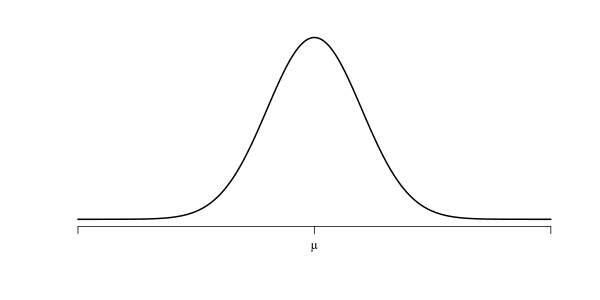
\includegraphics[width=10cm]{normal_dist.png}
    \onslide<2>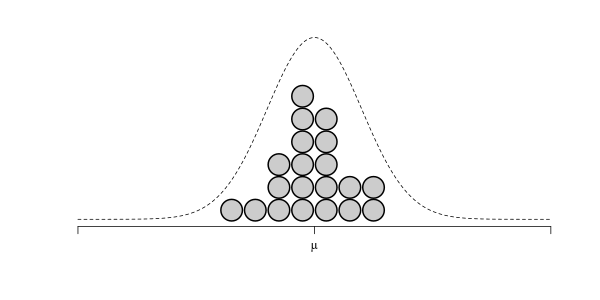
\includegraphics[width=10cm]{particle_dist.png}
  \end{overprint}
     
\end{frame}


\begin{frame}{Simple Example of Particle Filter}

  A bus driving down a one dimensional road.
  \onslide<+->

  \begin{itemize}[<+- | alert@+>]
  \item Start with an imaginary fleet
  \item Let each bus drive along the road and end up somewhere
  %\item Add some noise \ldots 
  \item Ask bus where it (thinks it) actually is
  \item Weight imaginary buses by distance to the real one
  \item Take a weighted sample (with replacement) to generate a new fleet
  \end{itemize}
  
  \begin{overprint}
    \onslide<2>
    \centering
    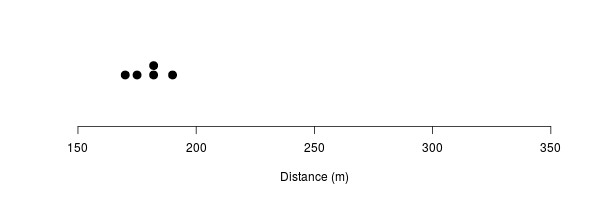
\includegraphics[width=0.8\textwidth]{figs/pf1-frame1.png}
    %\onslide<3>
    %\centering
    %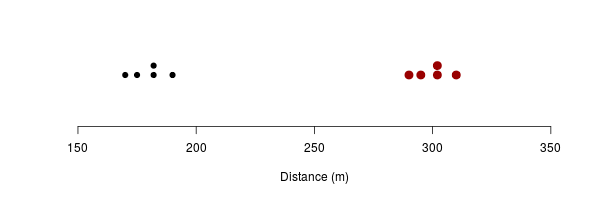
\includegraphics[width=0.8\textwidth]{figs/pf1-frame2.png}
    \onslide<3>
    \centering
    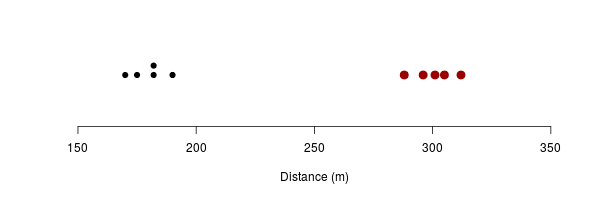
\includegraphics[width=0.8\textwidth]{figs/pf1-frame3.png}
    \onslide<4>
    \centering
    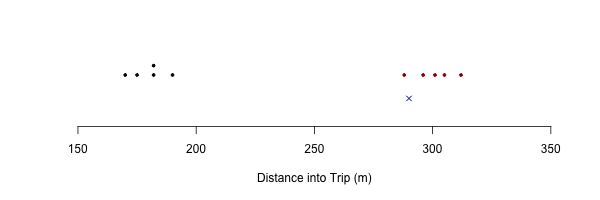
\includegraphics[width=0.8\textwidth]{figs/pf1-frame4.png}
    \onslide<5>
    \centering
    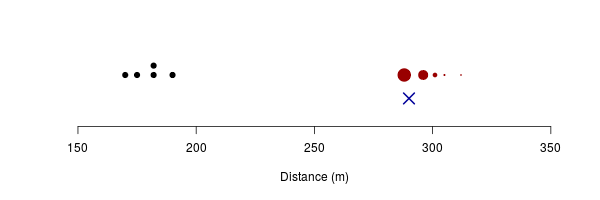
\includegraphics[width=0.8\textwidth]{figs/pf1-frame5.png}
    \onslide<6->
    \centering
    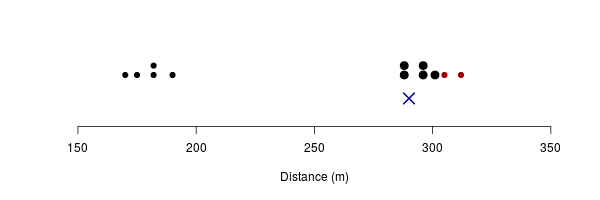
\includegraphics[width=0.8\textwidth]{figs/pf1-frame6.png}
  \end{overprint}

  \onslide<+->
\end{frame}


\begin{frame}{Real Example}
  Buses actually travel along fixed routes.
  
  \onslide<2->
  Route 049, Henderson -- Britomart:
  
  {\centering
  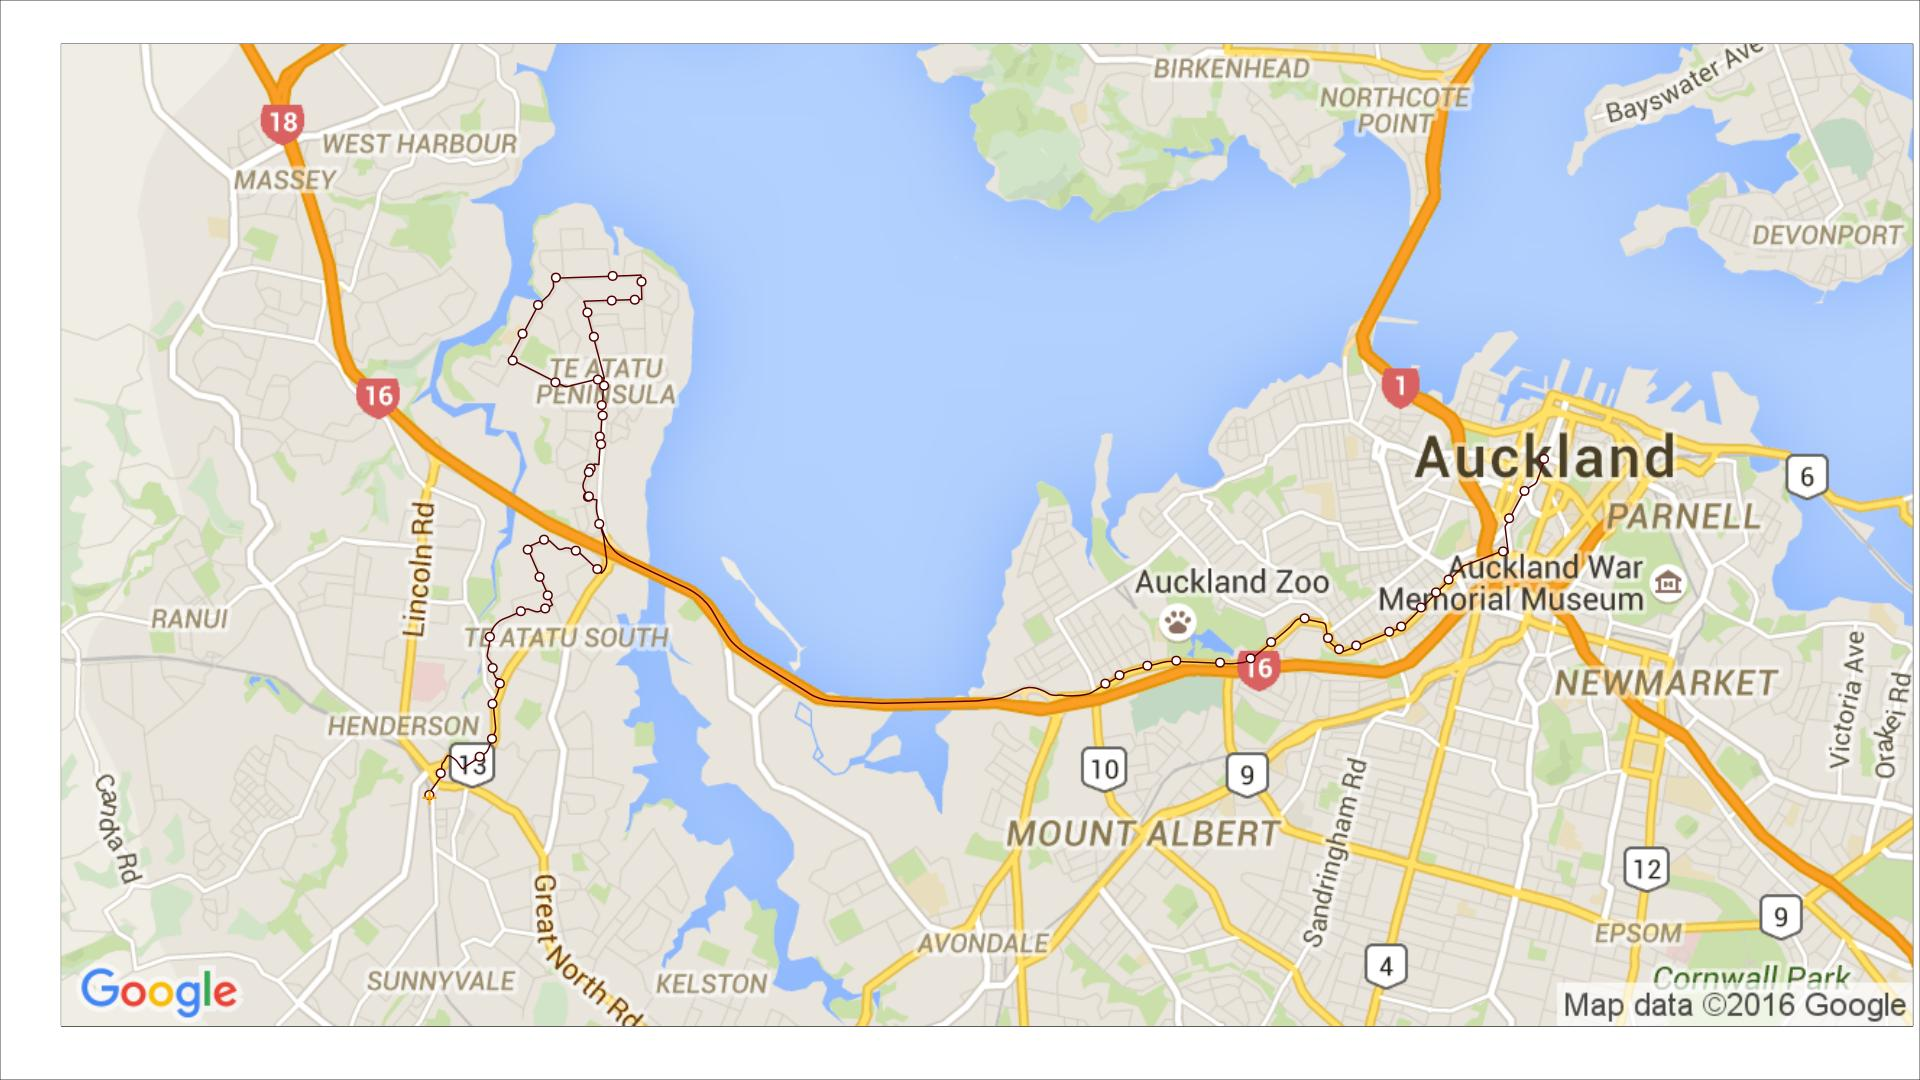
\includegraphics[width=\textwidth]{pf/particle_map001.jpg}}

  \footnotesize\url{https://www.stat.auckland.ac.nz/~tell029/phd/animations/route049.gif}

\end{frame}


\begin{frame}[standout]
  Thank you!
\end{frame}



\end{document}
